\documentclass{simple}

\title[CTF]{CTF: One for All. And More for Me}
\institute{UBB Avengers + UPB Justice League = $<$3}
\author[Răzvan Deaconescu]{Răzvan Deaconescu \\
razvan.deaconescu@upb.ro}
\date{27 mai 2021}

\begin{document}

\frame{\titlepage}

\begin{frame}{}
  \centering
  \LARGE
  Care este sensul vieții?
\end{frame}

\begin{frame}{}
  \centering
  \LARGE
  42 \\
  \LARGE
  n-are sens \\
  \LARGE
  perpetuarea \\
  \LARGE
  Singurul sens al vieții e să-i găsești un sens.
\end{frame}

\begin{frame}{Păzea!}
  \centering
  \url{https://forms.gle/q5UYS6ANcTKt7eLH7}
\end{frame}

\begin{frame}{Drive}
  \centering
  \pause
  \vspace{0.5cm}
  \Large{autonomy} \\
  \pause
  \vspace{0.5cm}
  \Large{mastery} \\
  \pause
  \vspace{0.5cm}
  \Large{purpose} \\
  \pause
  \vspace{0.5cm}
  \hfill \textit{Daniel Pink, Drive (2009)}
\end{frame}

\begin{frame}{Drive}
  \centering
  \vspace{0.5cm}
  \Large{\textbf{autonomy}} \\
  \vspace{0.5cm}
  \Large{\textbf{mastery}} \\
  \vspace{0.5cm}
  \Large{purpose} \\
  \vspace{0.5cm}
  \hfill \textit{Daniel Pink, Drive (2009)}
\end{frame}

\begin{frame}{Road to Autonomy and Mastery}
  \centering
  \pause
  \vspace{0.5cm}
  \Large{read / watch} \\
  \pause
  \vspace{0.5cm}
  \Large{learn} \\
  \pause
  \vspace{0.5cm}
  \Large{do} \\
  \pause
  \vspace{0.5cm}
  \Large{repeat} \\
  \pause
  \vspace{0.5cm}
  \Large{tell} \\
  \pause
  \vspace{0.5cm}
  \Large{create}
\end{frame}

\begin{frame}{Zen}
  To follow the path: \\
  look to the master, \\
  follow the master, \\
  walk with the master, \\
  see through the master, \\
  become the master.
\end{frame}

\begin{frame}{\textbf{O} cale: CTF}
  \centering
  \pause
  \vspace{0.5cm}
  \Large{Capture the Flag} \\
  \pause
  \vspace{0.5cm}
  \Large{competiție} \\
  \pause
  \vspace{0.5cm}
  \Large{echipă} \\
  \pause
  \vspace{0.5cm}
  \Large{securitate} \\
  \pause
  \vspace{0.5cm}
  \Large{premii și glorie}
\end{frame}

\begin{frame}{De ce CTF / Securitate?}
  \begin{figure}[!htbp]
    \centering
    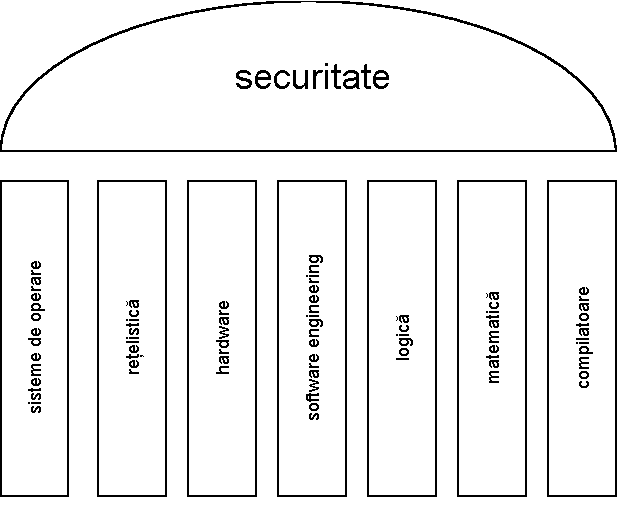
\includegraphics[width=0.8\textwidth]{img/security-deps.pdf}
  \end{figure}
\end{frame}

\begin{frame}{Povestea mea}
  \centering
  \pause
  \vspace{0.3cm}
  \textit{It was then I decided to take the initiative and invent the Internet.} \\
  \pause
  \vspace{0.3cm}
  Nu sunt la bază om de securitate. Sunt om de sisteme de operare / low-level. \\
  \pause
  \vspace{0.3cm}
  am aflat de la un student plecat la VUA de CTF-uri \\
  \pause
  \vspace{0.3cm}
  io.smashthestack.org \\
  \pause
  \vspace{0.3cm}
  curs de securitate (\textit{Operating Systems Security}) \\
  \pause
  \vspace{0.3cm}
  echipă de CTF \\
  \pause
  \vspace{0.3cm}
  Security Summer School \\
  \pause
  \vspace{0.3cm}
  organizare CTF-uri studențești \\
  \pause
  \vspace{0.3cm}
  proiecte de iOS security
\end{frame}

\begin{frame}{Ce-a însemnat pentru mine}
  \centering
  \pause
  \vspace{0.5cm}
  răbdare \\
  \pause
  \vspace{0.5cm}
  organizare echipă \\
  \pause
  \vspace{0.5cm}
  resurse colaborative (wiki, Google Drive, GitHub) \\
  \pause
  \vspace{0.5cm}
  creativitate
\end{frame}

\begin{frame}{Nu știu dacă mă pricep. E de mine?}
  \begin{figure}[!htbp]
    \centering
    
\includegraphics[width=0.8\textwidth]{img/yes-yes-yellow.jpg}
  \end{figure}
\end{frame}

\begin{frame}{But why?}
  \centering
  \pause
  \vspace{0.5cm}
  \Large{autonomy} \\
  \pause
  \vspace{0.5cm}
  \Large{mastery} \\
  \pause
  \vspace{0.5cm}
  \Large{tehnic, netehnic} \\
  \pause
  \vspace{0.5cm}
  \Large{nu e despre securitate, e despre învățare, provocare, îmbunățire}
\end{frame}

\begin{frame}{CTF Demo}
  \centering
  SSS Qualifiers, Web
\end{frame}

\begin{frame}{De unde încep?}
  \begin{itemize}
    \item picoCTF: \url{https://picoctf.org/}
    \item OverTheWire: \url{https://overthewire.org/wargames/}
    \item Security Summer School: \url{https://security.cs.pub.ro/summer-school/wiki/}
    \item \url{https://ctftime.org/}
  \end{itemize}
\end{frame}

\begin{frame}{And then?}
  \centering
  \pause
  \vspace{0.5cm}
  \Large{rezolvă challenge-uri} \\
  \pause
  \vspace{0.5cm}
  \Large{învață} \\
  \pause
  \vspace{0.5cm}
  \Large{spune și altora} \\
  \pause
  \vspace{0.5cm}
  \Large{\textbf{creează}}
\end{frame}

\begin{frame}{}
  \centering
  \LARGE
  Have fun and happy hacking, cracking, breaking, smashing, \textbf{learning}, \textbf{creating}!
\end{frame}

\begin{frame}{Resurse}
  \begin{itemize}
    \item slide-urile prezentării: \url{https://www.slideshare.net/razvandeaconescu/}
    \item cod sursă prezentare: \url{https://github.com/razvand/slides}
    \item Security Summer School: \url{https://security.cs.pub.ro/summer-school/wiki/}
    \item resurse agregate de wargames / CTF: \url{https://zaratec.github.io/ctf-practice/}
    \item alte resurse agregate de wargames / CTF: \url{https://fareedfauzi.gitbook.io/practice-ctf-list/}
    \item planificare CTF-uri: \url{https://ctftime.org/}
  \end{itemize}
\end{frame}

\end{document}
